\documentclass[a4paper, 12pt]{article}
\usepackage{pmgraph}
\usepackage[a4paper,portrait, margin=2.5cm]{geometry}
\usepackage[normalem]{ulem}
\usepackage[swedish,english]{babel}
\usepackage{graphicx,here,times,tabularx,rotating}
\usepackage{multicol}
\usepackage{float}
\usepackage{amssymb}
\usepackage{amsthm}
\usepackage{amsmath}
\usepackage[bottom]{footmisc}
\usepackage{physics}
\usepackage{bbm}
\usepackage{gensymb}
\usepackage{hyperref}
\usepackage[export]{adjustbox}
\usepackage[nottoc]{tocbibind}
\usepackage[toc,page]{appendix}
\usepackage{lipsum}
\usepackage{framed,xcolor}
\usepackage{libertine}
\usepackage{algorithm2e}
\usepackage{bm}% bold math
\usepackage[colorinlistoftodos]{todonotes}
\usepackage[utf8]{inputenc}
\usepackage{pgfplots}
\usepackage{tikz}
\usetikzlibrary{arrows}




\newcommand{\HRule}{\rule{\linewidth}{0.5mm}} % Defines a new command for the horizontal lines, change thickness here
\newcommand{\note}[1]{{\color{red}\textbf{#1} } }



\begin{document}


\pagenumbering{gobble}
%%%%%%%%%%%%%%%%%%%%%%%%%%%%%%%%%%%%%%%55
\begin{titlepage}


\center % Center everything on the page
 
 
 
 
%----------------------------------------------------------------------------------------
%	HEADING SECTIONS
%----------------------------------------------------------------------------------------

\textsc{\LARGE Uppsala University}\\[1.5cm] % Name of your university/college
\textsc{\Large Degree Project D in Computational Science, 30c}\\[0.5cm] % Major heading such as course name
\textsc{\large Department of Physics and Astronomy\\ Division of Material stuff?}\\[0.5cm] % Minor heading such as course title

%----------------------------------------------------------------------------------------
%	TITLE SECTION
%----------------------------------------------------------------------------------------

\HRule \\[0.4cm]
{ \huge \bfseries Holonomic optimal control for qudits}\\[0.4cm] % Title of your document
\HRule \\[1.5cm]
 
%----------------------------------------------------------------------------------------
%	AUTHOR SECTION
%----------------------------------------------------------------------------------------

\begin{minipage}{0.4\textwidth}
\begin{flushleft} \large
\emph{Author:}\\
Tomas \textsc{André} % Your name
\end{flushleft}
\end{minipage}
~
\begin{minipage}{0.4\textwidth}
\begin{flushright} \large
\emph{Supervisor:} \\
Erik \textsc{Sjöqvist} \\
\emph{Subject reader:} \\
Martin \textsc{Almquist} %% Supervisor's Name
\end{flushright}
\end{minipage}\\[2cm]

% If you don't want a supervisor, uncomment the two lines below and remove the section above
%\Large \emph{Author:}\\
%John \textsc{Smith}\\[3cm] % Your name

%----------------------------------------------------------------------------------------
%	DATE SECTION
%----------------------------------------------------------------------------------------

{\large \today}\\[2cm] % Date, change the \today to a set date if you want to be precise

%----------------------------------------------------------------------------------------
%	LOGO SECTION
%----------------------------------------------------------------------------------------


\includegraphics[scale = 0.11]{figures/uulogga.png}\\[1cm] % Include a department/university logo - this will require the graphicx package
 
%----------------------------------------------------------------------------------------

\vfill % Fill the rest of the page with whitespace

\end{titlepage}
%%%%%%%%%%%%%%%%%%%%%%%%%%%%%%%%
\newpage

\begin{abstract}1
    Engelskt abstrakt
\end{abstract}

\bigskip

\bigskip

\bigskip

\bigskip

\begin{otherlanguage}{swedish}
\begin{abstract}
    Svenskt abstrakt
  
\end{abstract}
\end{otherlanguage}


\newpage
\tableofcontents
\newpage
\pagenumbering{arabic}

Test! Här är några relevant källor! \cite{NHQC},\cite{morris},\cite{qudit}

\section{Introduction}
%The emerging field of quantum technology has many promising applications, one of them is quantum computation (QC), which currently is a very active area of research. Quantum computers make use of quantum mechanical effects such as superposition, entanglement, and interference to design powerful algorithms. These algorithms could be used to solve some hard problems which would not be  possible to solve using classical computation, such as efficient prime-number factoring [1]. It can also be used to reduce the time complexity of some commonly used algorithms [2]. Current quantum computers are very susceptible to decoherence and noise, and thus will not have any commercial use any time soon, but stand as an important proof of concept. 
The most common model for quantum computation is the circuit model, which is analogous to the classical circuits used for classical computers. Gates are replaced by unitary transformations (quantum gates) and bits by qubits. To achieve the computational advantage it is important to construct robust, noise-resilient quantum gates. A good candidate for this is holonomic quantum computation [3,4], which is based on the Berry phase [5] and its non-Abelian and/or non-adiabatic generalizations [6,7,8]. These methods are only dependent on the geometry of the system and thus are resilient to local errors in the dynamical evolution.


The idea that elements of computation should be limited to two-dimensional qubits is sort of an arbitrary choice that most likely rose out of convenience due to binary logic. So why binary logic? It is simply the easiest non-trivial example, in binary things can be either $1$ or $0$, {\tt True} or {\tt False}, \textbf{on} or \textbf{off}. Due to its simplicity, it is no wonder that this is how the first computer was designed. But are we limited to bits? As early as 1840 a mechanical trenary (three-valued logic) calculation device was built by Thomas Fowler [9], and in 1958 the first electronic trenary computer was built by the Soviet Union [10]. Even though it had many advantages over the binary computer it never saw the same widespread success. There is nothing in theory that forbids a higher dimensional computational basis, even more so when it comes to quantum computers, where the implementation of the elements of computation already surpasses the simplicity of \textbf{on} and \textbf{off}. There are promising qudit results that show potential [11,12,13], and in the review article [14] a good overview of the field is given and further research into the topic is encouraged.

In this report we will show how to find a new geometric phase based scheme to implement qudits which could be more efficient than some current ones by making use of dark paths for increased parameter control and auxiliary states for increased fidelity. We do this by generalizing the idea of the scheme from [15]. The report is structured as follows. The background section is split into two parts where the first part serves as a quick introduction to the most important aspects of quantum mechanics as well as the commonly used notation. Then follows a part more concerned with quantum computation, quantum information, and some of the more advanced quantum mechanical concepts that those are built upon. Then the main results are shown, first an explicit example for the qutrit and then how it generalizes in higher dimensions. The report ends with conclusions and a brief outlook.




\section{Background}
%The Background consists of a quick introduction to the most important quantum mechanical concepts and notation. Readers familiar with quantum mechanics may skip it. The second part explores the fundamentals of quantum computation and 

\subsection{Basic quantum mechanics, part I}
This part offers a quick introduction to the necessary  quantum mechanics for readers whom are not familiar with the subject. The section contains nothing relevant for later parts of the thesis and can be safely skipped. For a more complete introduction I suggest chapter 1 of Sakurai.

\subsubsection{Kets, Bras and Operators}
When talking about Quantum mechanics the term \textbf{quantum state}, or more likley just state, is mentioned a lot. A quantum mechanical state is represented by a \textbf{ket}, an complex-valued vector with either finite or infinite entries. Closely related to the ket is the \textbf{bra}, which is the corresponding vector to the ket in the dual space, or more simply, the hermitian conjugate of the ket, see Equation \ref{eq:ket}.
\begin{equation}
\label{eq:ket}
\ket{\psi} = \begin{pmatrix}
a_1 \\ a_2 \\ \vdots \\ a_n
\end{pmatrix},\;
\bra{\psi} = (\ket{\psi})^{\dagger} = (a_1^{*}, a_2^{*}, \dots, a_n^{*}),\; a_1,a_2,\dots,a_n \in \mathbb{C}
\end{equation} 
An arbitrary ket can be rewritten as a linear combination of its eigenkets that span the same space, $\ket{\psi} = \sum_i a_i\ket{i}$ The coefficient is know as the probability amplitude, and $|a_i|^2$ corresponds to the probability to find the state in the $i$th state. 
The inner product of two quantum states is simply written as 
$\bra{\varphi}\ket{\psi} = (\bra{\varphi}\ket{\psi})^\dagger \in \mathbb{C}$. 
An operator can act on a quantum state and corresponds to multiplication with a matrix, and will always yield a new state, ket. 
\begin{equation}
\hat{O}\ket{\psi} = \ket{\psi'}
\end{equation}
Operators are often written in terms of of kets and bras, for example and operator which takes the state $\ket{1}$ and returns the state $\ket{2}$ is written as
\begin{equation}
(\ket{2}\bra{1})\ket{1} = \ket{2}\bra{1}\ket{1} = \ket{2}(\bra{1}\ket{1}) = (\bra{1}\ket{1})\ket{2} = 1 \ket{2} = \ket{2}
\end{equation}
or a identity $2\times 2$ matrix would be
\begin{equation}
 \begin{pmatrix}
 1 & 0 \\ 0 & 1
 \end{pmatrix} = \ket{1}\bra{1} + \ket{2}\bra{2} 
\end{equation}
and so on. An operator for a physical measurable quantity is called an observable.

\subsubsection{Measurements and Observables and Uncertainty}
A quantum mechanical measurement ''breaks'' the superposition of a quantum states and shifts it into a eigenstate of the observable,
\begin{equation}
\ket{\psi} \longrightarrow \ket{i}
\end{equation}
the probability to find the $i$th eigenstate is $|a_i|^2$. 
In quantum mechanics the relation $AB - BA = 0$,where $A$ and $B$ are operators, does not generally hold. This is due to the uncommutative nature of quantum mechanics, it relates to uncertainty but it also required since it a can realize a more complex mathematical structure. The fact that matrices are non-commutative are not surprising, and since operators can be represented by matrices this should not be that confusing. 
To make it more concrete to which degree two operators commute one can define  the commutator on operators $A,B$ as $[A,B] = AB - BA$, which is zero for commuting operators and non-zero otherwise. 
Observables which don't commute are called incompatible observables, a well know pair of incompatible observables are position and momentum, $\mathbf{x}$ and $\mathbf{p}$, which can not be measured to arbitrary precision, this is due to the fact that $[\mathbf{x},\mathbf{p}] \neq 0$. So for two incompatible observables the general uncertainty the measurements will be limited by \note{uncertainty relation here.} 

\subsubsection{Time evolution and the Schrödinger equation}

\subsection{Quantum Computation and Quantum Information theory, part 2}

\subsubsection{The Qubit}
A classical bit is a binary system which, so it can occupy two states, either 0 or 1. So with $n$ bits there is $2^n$ possible states that can be represented, but only one at a time.

A qubit is a quantum state that is in a superposition of $\ket{0}$ and $\ket{1}$, so a general qubit would have the form
\begin{equation}
\label{eq:qubit}
\ket{\psi} = \alpha\ket{0} + \beta\ket{1},\,\alpha,\beta \in \mathbb{C},\, |\alpha|^2 + |\beta|^2 = 1.
\end{equation}
The qubit is no limited to 0 and 1, but can exist in a linear combination of those states. When a measurement is performed the qubit will collapse into $\ket{1}$ or $\ket{2}$ with probability $|\alpha|^2$ and $|\beta|^2$ respectively. A consequence of superposition is that $n$ qubits can represent $2^n$ states simultaneously.

The combined state of two qubits $\ket{\psi_1}$ and $\ket{\psi_2}$ is given by 
\begin{equation}
\ket{\psi_1} \otimes \ket{\psi_2} = (\alpha_1\ket{0} + \beta_1\ket{1})\otimes(\alpha_2\ket{0} + \beta_2\ket{1})
\end{equation}
the tensor product is often omitted and one would write $\ket{\psi_1} \otimes \ket{\psi_2} = \ket{\psi_1}\ket{\psi_2} = \ket{\psi_1, \psi_2}$.

Some of the common qubit gates are the Pauli gates $X,Y,Z$, the Hadamard gate $H$, and the T-gate $T$.





\subsubsection{Information stuff}

\subsubsection{Universal computation}

\subsubsection{Holonomic Quantum Computation}



\subsection{Lambda system}
A traditional $\Lambda$-system is a quantum mechanical system with two decoupled 'ground states' and one 'excited state' coupled to both ground states. Such a state with two ground state could realize a qubit by letting the ground state act as $\ket{0}$ and $\ket{1}$.

\begin{figure}[H]
    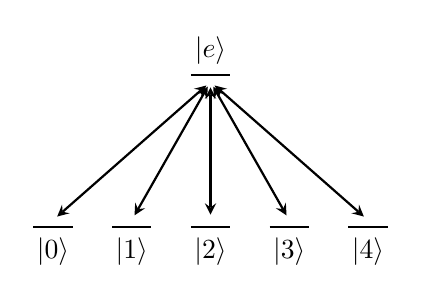
\begin{tikzpicture}[
      scale=0.5,
      level/.style={thick},
      virtual/.style={thick,densely dashed},
      trans/.style={thick,<->,shorten >=2pt,shorten <=2pt,>=stealth},
      classical/.style={thin,double,<->,shorten >=4pt,shorten <=4pt,>=stealth}]
      
    % Draw the energy levels.
    \draw[level] (6cm,0em) -- (7cm,0em) node[midway,above] {$\ket{e}$};
    \draw[level] (2cm,-11em) -- (3cm,-11em) node[midway,below] {$\ket{0}$};
    \draw[level] (4cm,-11em) -- (5cm,-11em) node[midway,below] {$\ket{1}$};
    \draw[level] (6cm,-11em) -- (7cm,-11em) node[midway,below] {$\ket{2}$};
    \draw[level] (8cm,-11em) -- (9cm,-11em) node[midway,below] {$\ket{3}$};
    \draw[level] (10cm,-11em) -- (11cm,-11em) node[midway,below] {$\ket{4}$};
    % Draw the transitions.
    
    \draw[trans] (6.5cm,-0.5em) -- (2.5cm,-10.5em) node[midway,left] {};
    \draw[trans] (6.5cm,-0.5em) -- (4.5cm,-10.5em) node[midway,left] {};
    \draw[trans] (6.5cm,-0.5em) -- (6.5cm,-10.5em) node[midway,left] {};
    \draw[trans] (6.5cm,-0.5em) -- (8.5cm,-10.5em) node[midway,left] {};
    \draw[trans] (6.5cm,-0.5em) -- (10.5cm,-10.5em) node[midway,left] {};
    %\draw[trans] (1cm,-2em) -- (2.5cm,8em) node[midway,left] {\ome{1}};
    %\draw[trans] (3.5cm,8em) -- (5cm,-8em) node[midway,right] {\Om{2}};
    %\draw[classical] (4.5cm,-8em) -- (1.5cm,-5em) node[midway,below] {\Ga{}};
    \end{tikzpicture}
    
    \caption{test figure}
\end{figure}

alfa $=$ $\frac{\pi}{2}\sin^{2}(\frac{\pi t}{T})$

beta $=$ $\eta(1 - \cos( \frac{\pi}{2}\sin^{2}(\frac{\pi t}{T}) ))$

alfa' $=$ $\frac{\pi^2}{2T}\sin(\frac{2\pi t}{T})$

beta' $=$ $\frac{\eta\pi^2}{2T}\sin(\frac{2\pi t}{T})\sin(\frac{\pi}{2}\sin^{2}(\frac{\pi t}{T}))$

\begin{equation*}
\Omega(t) = 2( (\frac{\eta\pi^2}{2T}\sin(\frac{2\pi t}{T})\sin(\frac{\pi}{2}\sin^{2}(\frac{\pi t}{T})))\cot(\frac{\pi}{2}\sin^{2}(\frac{\pi t}{T}))\sin(\eta(1 - \cos( \frac{\pi}{2}\sin^{2}(\frac{\pi t}{T}) )))
\end{equation*}
\begin{equation*}
+ \eta(1 - \cos( \frac{\pi}{2}\sin^{2}(\frac{\pi t}{T}) ))\cos(\eta(1 - \cos( \frac{\pi}{2}\sin^{2}(\frac{\pi t}{T}) ))) )
\end{equation*}



\subsection{Coupled excited states}
Hamiltonian of a ''double'' tripod
\begin{equation}
H(t) = \sum^2_{i = 1} \sum^3_{j = 1} \omega_{ij} \ket{j}\bra{e_i} + \text{h.c}
\end{equation}

Find dark states $H(t)\ket{d} = 0\ket{d} $ on form $\ket{d} = \sum_{k = 1}^3 d_k \ket{k}$
Result

\begin{equation}
\begin{aligned} &
d_1 = \frac{1}{\omega^{*}_{11}} \left(\omega^{*}_{12}\omega^{*}_{23}  - \omega^{*}_{13}\omega^{*}_{22} \right)
\\ &
d_2 = \frac{\omega^{*}_{13}\omega^{*}_{21}}{\omega^{*}_{11}} - \omega^{*}_{23}
\\ &
d_3 = \omega^{*}_{22} - \frac{\omega^{*}_{12}\omega^{*}_{21}}{\omega^{*}_{11}}
\end{aligned}
\end{equation}

Bright state $\bra{b}\ket{d} = 0$ 

\begin{equation}
\begin{aligned} &
\ket{b_1} = \omega_{11}\ket{1} + \omega_{12}\ket{2} + \omega_{13}\ket{3}
\\ &
\ket{b_2} = \omega_{21}\ket{1} + \omega_{22}\ket{2} + \omega_{23}\ket{3}
\end{aligned}
\end{equation}
Check if $\bra{b_1}\ket{b_2} = 0$? Holds if $\omega_{11} = -\frac{1}{\omega^{*}_{21}}\left(\omega^{*}_{12}\omega_{22} + \omega_{13}\omega^{*}_{23} \right)$


Change basis, 
\begin{equation}
T = \begin{pmatrix}
1 & 0 & 0 & 0 & 0 \\
0 & 1 & 0 & 0 & 0  \\
0 & 0 & \omega_{11} & \omega_{21} & d_1  \\
0 & 0 & \omega_{12} & \omega_{22} & d_2  \\
0 & 0 & \omega_{13} & \omega_{23} & d_3  \\
\end{pmatrix}
\end{equation}

New hamiltonian in $\{\ket{e_1}, \ket{e_2}, \ket{b_1}, \ket{b_2}, \ket{d} \}$ is 
\begin{equation}
H_d(t) = T^\dagger H(t) T = \left(\sum_{j = 1}^2 \sum_{k = 1}^3 \left( \omega_{jk} \right)^2 \ket{b_j}\bra{e_j}\right) + \left[\omega_{11}\omega_{12} + \omega_{12}\omega_{22} + \omega_{13}\omega_{23} \right]\left(\ket{b_2}\bra{e_1} + \ket{b_1}\bra{e_2}\right)\; + \;\text{h.c} 
\end{equation} 
\note{Double check this calculation.}


Subspace is  $\{\ket{e_1}, \ket{e_2}, \ket{b_1}, \ket{b_2} \}$ since $\ket{d}$ is decoupled.\\
Simplify notation, $\Omega_j = \sum_{k = 1}^3 \omega_{jk}^2$ and $\Gamma = \omega_{11}\omega_{12} + \omega_{12}\omega_{22} + \omega_{13}\omega_{23}$ now Hamiltonian looks like 
\begin{equation}
H_d = \sum_{j = 1}^2 \Omega_j \ket{b_j}\bra{e_j} + \Gamma\left(\ket{b_2}\bra{e_1} + \ket{b_1}\bra{e_2} \right) + \; \text{h.c}
\end{equation}
\\
Now find a ''dark path'' $\ket{D_i(t)}$ such that $\bra{D_i(t)}H_d(t)\ket{D_i(t)} = 0$, for $i = 1,2$
\\ Set
\begin{equation}
\begin{aligned} &
 \ket{D_1} = a_1\ket{b_1} + a_2\ket{3} + a_3\ket{e_1}
 \\ &
 \ket{D_2} = c_1\ket{b_2} + c_2\ket{3} + c_3\ket{e_2}
 \end{aligned}
\end{equation}

and


\vspace{3cm}
NEW TRY

\begin{equation}
H(t) = \sum^2_{i = 1} \sum^3_{j = 1} \omega_{ij} \ket{j}\bra{e_i} + \text{h.c}
\end{equation}

New dark state 
\begin{equation}
\ket{d} = d_1\ket{1} + d_2\ket{2}
\end{equation}
with $d_1 = -(\omega_{12}^{*} + \omega_{22}^{*})$, $d_2 = (\omega_{11}^{*} + \omega_{21}^{*})$
\note{There exists no dark state on this form ($d_1 = d_2 = 0$)}

bight state 
\begin{equation}
\ket{b} = -d_2^{*}\ket{1} + d_1^{*}\ket{2}
\end{equation}

\textbf{CRITERA?} $\omega_{11}\omega_{22} = \omega_{12}\omega_{21} \implies \frac{\omega_{11}}{\omega_{12}} = \frac{\omega_{21}}{\omega_{22}}$

change basis to $\{e_1, e_2, 3, b, d\}$
\begin{equation}
T = \begin{pmatrix}
1 & 0 & 0 & 0 & 0 \\
0 & 1 & 0 & 0 & 0  \\
0 & 0 & 0 & -d_2^{*} & d_1  \\
0 & 0 & 0 & d_1^{*} & d_2  \\
0 & 0 & 1 & 0 & 0  \\
\end{pmatrix}
\end{equation}


New hamiltonian 
\begin{equation}
H_d = \left(\sum_{j = 1}^{2} \omega_{j3}\ket{3}\bra{e_j} + \sigma_j\ket{b}\bra{e_j} \right) + \text{h.c}
\end{equation}
with 
$$
\sigma_1 = \omega_{12}d_1^{*} - \omega_{11}d_2^{*} = -\omega_{12}(\omega_{12} + \omega_{22}) - \omega_{11}(\omega_{11} + \omega_{21})
$$
$$
\sigma_2 = \omega_{21}d_1^{*}-\omega_{12}d_2^{*} = -\omega_{23}(\omega_{12} + \omega_{22}) - \omega_{12}(\omega_{11} + \omega_{21})
$$
\\
Now find a ''dark path'' $\ket{D_i(t)}$ such that $\bra{D_i(t)}H_d(t)\ket{D_i(t)} = 0$, for $i = 1,2$
\\ Set
\begin{equation}
\begin{aligned} &
 \ket{D_1} = a_1\ket{b} + a_2\ket{3} + a_3\ket{e_1}
 \\ &
 \ket{D_2} = c_1\ket{b} + c_2\ket{3} + c_3\ket{e_2}
 \end{aligned}
\end{equation}
Assume that $\ket{b_2} = \Delta\ket{b_1}$

\begin{equation}
\begin{aligned} &
 \ket{D_1} = \cos\alpha\cos\beta (((e^{-i\varphi})))\ket{b_1} - \cos\alpha\sin\beta\ket{3} - i\sin\alpha\ket{e_1}
 \\ &
 \ket{D_2} = \cos\alpha\cos\beta (((e^{-i\varphi})))\ket{b_2} - \cos\alpha\sin\beta\ket{3} - i\sin\alpha\ket{e_2}
 \end{aligned}
\end{equation}

then $\bra{D_1}\ket{D_2} = 0 \implies \bra{b_1}\ket{b_2} = - \tan^2\beta \implies \Delta = -i\tan\beta$ 
\begin{equation}
\begin{aligned}&
\bra{D_i}H_d\ket{D_i} = \left[\sigma_1^{*} + \sigma_2^{*} - \sigma_i\right]\Delta_i\cos\beta + \omega_{i3}\sin\beta = 0
\\ &
\implies \omega_{i3} = \Delta_i(\sigma_i - \sigma_1^{*} - \sigma_2^{*})\cot\beta
\end{aligned}
\end{equation}



\vspace{3cm}

NEW NEW TRY!\\

\begin{equation}
H(t) = \sum^2_{i = 1} \sum^3_{j = 1} \omega_{ij} \ket{j}\bra{e_i} + \text{h.c}
\end{equation}

Dark state

\begin{equation}
\begin{aligned} &
d_1 = -\left(\omega^{*}_{22} + \frac{\omega^{*}_{12}\omega^{*}_{23}}{\omega^{*}_{13}} \right)
\\ &
d_2 = \left(\omega^{*}_{21} + \frac{\omega^{*}_{11}\omega^{*}_{23}}{\omega^{*}_{13}}\right)
\\ &
d_3 = \frac{1}{\omega^{*}_{13}}\left( \omega^{*}_{21}\omega^{*}_{12} - \omega^{*}_{11}\omega^{*}_{22}\right)
\end{aligned}
\end{equation}
bright state 
\begin{equation}
\ket{b} = -d_2^{*}\ket{1} + d_1^{*}\ket{2}
\end{equation}


\begin{equation}
H_d = \left(\sum_{j\ = 1}^{2} \omega_{j3}\ket{3}\bra{e_j} + \sigma_j\ket{b}\bra{e_j} \right) + \text{h.c}
\end{equation}

$$
\sigma_1 = -\frac{\omega_{23}}{\omega_{13}}\left(\omega_{12}^2 + \omega_{11}^2 \right) - \omega_{11}\omega_{21} - \omega_{12}\omega_{22}
$$
$$
\sigma_2 = -\frac{\omega_{23}}{\omega_{13}}\left(\omega_{12}\omega_{22} + \omega_{11}\omega_{21}\right) - \left(\omega_{12}^2 + \omega_{22}^2\right)
$$
Then computations follow as before with new coeffcients.
\newpage

\begin{equation}
H = \sum_{j = 1}^{2}\alpha_j \ket{\alpha_j}\bra{e_j} + \sum_{i = 1}^{2} \omega_{ji} \ket{i}\bra{e_j} + \;\text{h.c}
\end{equation}
in new basis
\begin{equation}
H_d = \sum_{j = 1}^2 -\alpha_j^2 - \sum_{i = 1}^{2}\omega_{ji}^{2}\ket{b_j}\bra{e_j} -(\omega_{11}\omega_{21} + \omega_{12}\omega_{22})(\ket{b_2}\bra{e_1} + \ket{b_1}\bra{e_2}) + \; \text{h.c}
\end{equation}
simplify 
\begin{equation}
H_d = \sum_{j = 1}^2 \sigma_j\ket{b_j}\bra{e_j} + \Gamma (\ket{b_2}\bra{e_1} + \ket{b_1}\bra{e_2}) + \; \text{h.c}
\end{equation}

\begin{equation}
\begin{aligned} &
 \ket{D_1} = \cos\alpha\cos\beta e^{-i\varphi_1}\ket{b_1} - \cos\alpha\sin\beta\ket{\alpha_1} - i\sin\alpha\ket{e_1}
 \\ &
 \ket{D_2} = \cos\alpha\cos\beta e^{-i\varphi_2}\ket{b_2} - \cos\alpha\sin\beta\ket{\alpha_2} - i\sin\alpha\ket{e_2}
 \end{aligned}
\end{equation}

\begin{equation}
\bra{D_1}\ket{D_2} = \cos^2\alpha \cos^2\beta e^{+i(\varphi_2 - \varphi_1)}\bra{b_1}\ket{b_2} == 0 \textbf{?}
\end{equation}
holds if
\begin{equation}
\bra{b_1}\ket{b_2} = \omega_{11}^{*}\omega_{21}^{} + \omega_{12}^{*}\omega_{22}^{} = 0
\end{equation}

\newpage

NEW, hopefully last, try

The system \begin{figure}[H]
    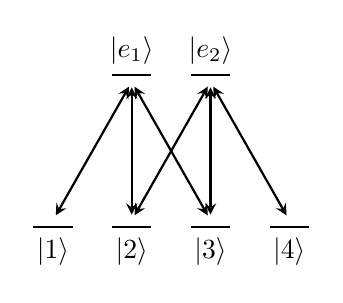
\begin{tikzpicture}[
      scale=0.5,
      level/.style={thick},
      virtual/.style={thick,densely dashed},
      trans/.style={thick,<->,shorten >=2pt,shorten <=2pt,>=stealth},
      classical/.style={thin,double,<->,shorten >=4pt,shorten <=4pt,>=stealth}]
      
    % Draw the energy levels.
    \draw[level] (6cm,0em) -- (7cm,0em) node[midway,above] {$\ket{e_1}$};    

    \draw[level] (4cm,-11em) -- (5cm,-11em) node[midway,below] {$\ket{1}$};
    \draw[level] (6cm,-11em) -- (7cm,-11em) node[midway,below] {$\ket{2}$};
    \draw[level] (8cm,-11em) -- (9cm,-11em) node[midway,below] {$\ket{3}$};
    \draw[level] (10cm,-11em) -- (11cm,-11em) node[midway,below] {$\ket{4}$};
    % Draw the transitions.
    
   
    \draw[trans] (6.5cm,-0.5em) -- (4.5cm,-10.5em) node[midway,left] {};
    \draw[trans] (6.5cm,-0.5em) -- (6.5cm,-10.5em) node[midway,left] {};
    \draw[trans] (6.5cm,-0.5em) -- (8.5cm,-10.5em) node[midway,left] {};

    
       
   
    \draw[trans] (8.5cm,-0.5em) -- (6.5cm,-10.5em) node[midway,left] {};
    \draw[trans] (8.5cm,-0.5em) -- (8.5cm,-10.5em) node[midway,left] {};
    \draw[trans] (8.5cm,-0.5em) -- (10.5cm,-10.5em) node[midway,left] {};


    \draw[level] (8cm,0em) -- (9cm,0em) node[midway,above] {$\ket{e_2}$};
    \end{tikzpicture}
    
    \caption{test figure}
\end{figure}

has a dark state $\ket{d}$ on the form 
\begin{equation}
\ket{d} = c_1\ket{1} + c_2\ket{2} + c_3\ket{3},\;\; |c_1|^2 + |c_2|^2 + |c_3|^2 = 1
\end{equation}

There exists two orthogonal bright states on the form 

\begin{equation}
\begin{aligned} &
\ket{b_1} = N_1 \left(x\ket{1} + c_2\ket{2} + c_3\ket{3} \right)
\\ &
\ket{b_2} = N_2 \left(-c_3^{*}\ket{2} + c_2^{*}\ket{3} \right)
\end{aligned}
\end{equation}

One can see that
$\bra{b_1}\ket{b_2} = \bra{d}\ket{b_1} 0$, find $x$ such that $\bra{d}\ket{b_1} = 0$.

After finding $x$ and normalizing the result is 
\begin{equation}
\begin{aligned}&
\ket{d} = c_1\ket{1} + c_2\ket{2} + c_3\ket{3}
\\ &
\ket{b_1} = \frac{|c_1|}{\sqrt{1-|c_1|^2}} \left(\left(c_1 - \frac{1}{c_1^{*}}\right)\ket{1} + c_2\ket{2} + c_3\ket{3} \right)
\\ &
\ket{b_2} =  \frac{1}{\sqrt{1-|c_1|^2}} \left(-c_3^{*}\ket{2} + c_2^{*}\ket{3} \right)
\end{aligned}
\end{equation}

The hamiltonian in the space spanned by $\{e_1, e_2, b_1, b_2, 4, d\}$ is given by 
\begin{equation}
H_d = \frac{\Omega_1(t)}{2}e^{-i\phi_1} \ket{b_1}\bra{e_1} + \frac{\Omega_2(t)}{2}e^{-i\phi_2} \ket{b_2}\bra{e_2} + \frac{\Omega_3(t)}{2}\ket{4}\bra{e_2} + \; \text{h.c}
\end{equation}

Two dark paths $\ket{D_i}$ exists such that  $\bra{D_i}H_d\ket{D_i} = 0, \; i=1,2$, on the form

\begin{equation}
\begin{aligned}&
\ket{D_1} = \alpha_1\ket{b_1} + \beta_1\ket{e_1}
\\&
\ket{D_2} = \alpha_2\ket{b_2} + \beta_2\ket{e_2} + \gamma\ket{4}
\end{aligned}
\end{equation}
A choice would be, given two functions, $u(0) = u(T) = v(0) = v(T) = 0$,
\begin{equation}
\begin{aligned}&
\alpha_1 = \cos u(t)
\\&
\beta_1 = e^{i(\phi_1 + \frac{\pi}{2})}\sin u(t)
\\&
\alpha_2 = \cos u \cos v e^{-i\phi_2}
\\&
\beta_2 = -i\sin u
\\&
\gamma = -\cos u\sin v
\end{aligned}
\end{equation}

the coeffcients of the dark state could be parametrized by 4 angles, $\chi, \xi, \theta, \varphi$ 

\begin{equation}
\begin{aligned}&
c_1 = e^{i\chi}\sin \theta \cos \varphi, 
\\&
c_2 = e^{i\xi} \sin \theta \sin \varphi,
\\&
c_3 = \cos \theta.
\end{aligned}
\end{equation}

Now to find the parameters $\Omega_1(t), \Omega_2(t), \Omega_3(t)$, this can be done by reverse engineering by solving the schrödinger equation for $\ket{D_1}, \ket{D_2}$, 

\begin{equation}
\begin{aligned}&
i\pdv{}{t}\ket{D_1(t)} = H_d\ket{D_1(t)}
\\&
i\pdv{}{t}\ket{D_2(t)} = H_d\ket{D_2(t)}
\end{aligned}
\end{equation}
a calculation yields
\begin{equation}
\begin{aligned}&
\Omega_1(t) = -2\dot{u}
\\ &
\Omega_2(t) = 2\left(\dot{v}\cot u\sin v + \dot{u}\cos v \right)
\\ &
\Omega_3(t) = 2\left(\dot{v}\cot u\sin v - \dot{u}\sin v \right)
\end{aligned}
\end{equation}

Split time evol. into two parts.
The relevant part of the time evolution operator is
\begin{equation}
\begin{aligned}&
U_1 = \ket{d}\bra{d} -i\ket{e_1}\bra{b_1} -i\ket{e_2}\bra{b_2},\; \phi_1 = \phi_2 = 0
\\&
U_2 = \ket{d}\bra{d} +ie^{i\gamma_1}\ket{b_1}\bra{e_1} +ie^{i\gamma_2}\ket{b_2}\bra{e_2},\; \phi_1 = -\gamma_1,\; \phi_2 = -\gamma_2
\end{aligned}
\end{equation}

The complete operator is then given by 
\begin{equation}
U = U_2U_1 = \ket{d}\bra{d} + e^{i\gamma_1}\ket{b_1}\bra{b_1} + e^{i\gamma_2}\ket{b_2}\bra{b_2}
\end{equation}
Then $U$ is unitary in the computational subspace $\{d,b_1,b_2\}$, since $UU^{\dagger} = U^{\dagger}U = \mathbbm{1}$ 


One can set $u(t) = \frac{\pi}{2}\sin^2\frac{\pi t}{T}$ and $v(t) = \eta\left[1 - \cos u(t)\right]$

Now $U$ can be determined by the 6(?) real parameters $\chi, \xi, \theta, \varphi, \gamma_1, \gamma_2$ as $U(\chi, \xi, \theta, \varphi, \gamma_1, \gamma_2)$ 







\newpage
\bibliographystyle{vancouver}
\bibliography{ref.bib}


\appendix






\end{document}